\documentclass[a4paper]{jsarticle}

\usepackage{otf}	%日本語化
\usepackage[dvipdfmx]{xcolor} %色
\usepackage{listings}	%プログラム埋め込み
\usepackage[dvipdfmx]{graphicx,xcolor} %jpeg/pngの挿入
\usepackage{here}

\lstset{
	language={C}, %プログラム言語
	basicstyle = \ttfamily\scriptsize, 	%標準の書体
	keywordstyle = {\color[cmyk]{0,1,0,0}},%キーワード(int, ifなど)の書体
	commentstyle = {\color[cmyk]{1,0.4,1,0}},%コメントの書体
	frame=tRBl, %フレームの指定
	framesep=10pt, %フレームと中身(コード)の間隔
	breaklines=false, %行が長くなった場合の改行
	linewidth=13cm, %フレームの横幅
	lineskip=-0.5ex, %行間の調整
	tabsize=2, %Tabを何文字幅にするかの指定
	numbers=left, %行番号を表示
	numbersep=20pt,
 	captionpos = b, %キャプションの場所("tb"ならば上下両方に記載)
	xleftmargin=2truecm,%左側の余白
}


\title{第13回 プログラミング応用レポート}
\author{15302114番 山下尚人}
\date{提出日:20年2月1日}

\begin{document}
\maketitle%タイトル

\section*{課題}
	\begin{itemize}
	\item 実行結果
		sizeを20にして実行した結果、以下のような実行結果が得られた。\\
		
		\lstinputlisting[caption=sizeが20での実行結果, label={lst:実行結果}, language={}]{./size20.log} 
		
		また、sizeを5000〜30000まで1000刻みで変更して実行した結果、次のようなグラフになった。\\
		図1はsizeとswapが呼び出された回数、図2はsizeと実行にかかった時間のグラフ。\\
		random average(赤線)は初期配列をバラバラにして、同じsizeで10回実行した平均の値。\\
		worst(青線)は初期配列を降順にした場合の、実行した値を使用している。
		
		\begin{figure}[H]
			\centering
			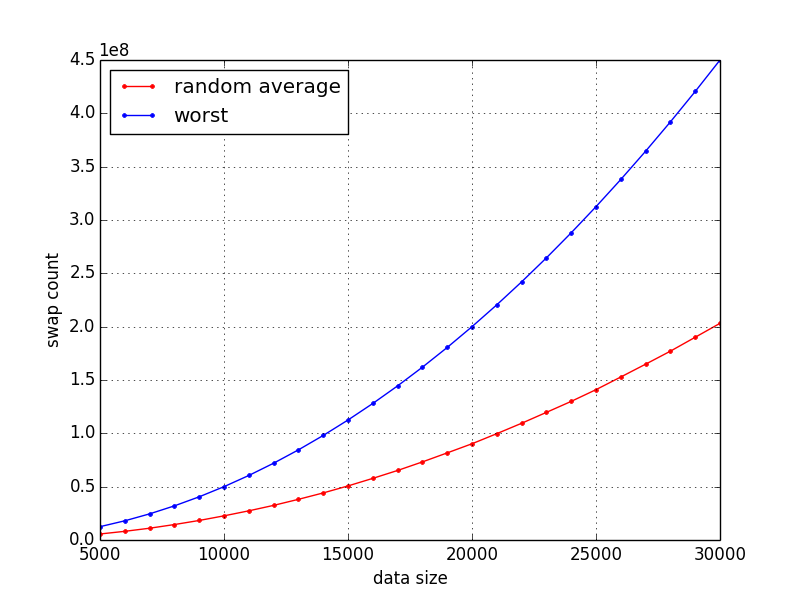
\includegraphics[width=13cm]{./fig1.png}
			\caption{sizeとswapが呼び出された回数}
			\label{fig:1}
		\end{figure}
		\begin{figure}[H]
			\centering
			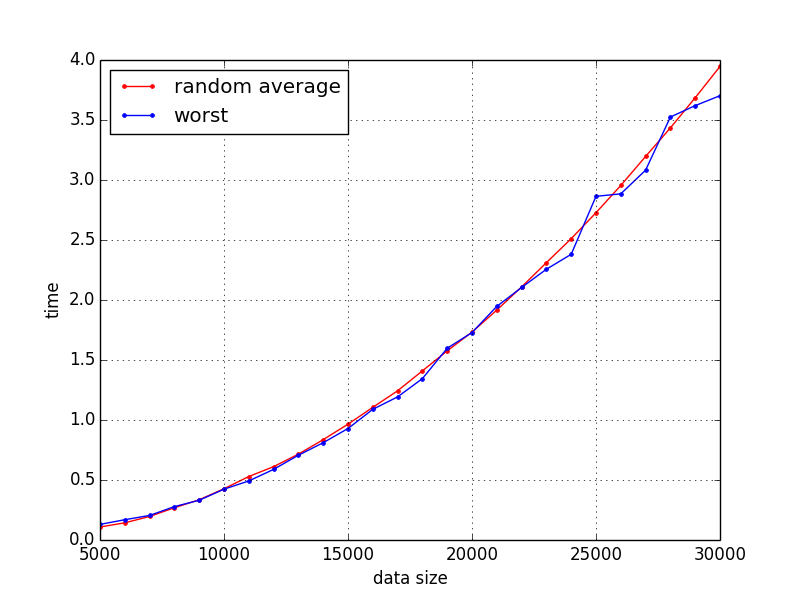
\includegraphics[width=13cm]{./fig2.png}
			\caption{sizeと実行にかかった時間}
			\label{fig:2}
		\end{figure}
		
	\end{itemize}
\end{document}
